\documentclass[11pt,a4paper]{article}

\usepackage[utf8]{inputenc}
\usepackage[T1]{fontenc}
\usepackage{lmodern}
\usepackage[margin=2.5cm]{geometry}
\usepackage{hyperref}
\usepackage{fancyvrb}
\usepackage{graphicx}

\hypersetup{colorlinks=true, urlcolor=blue}

\fvset{fontsize=\footnotesize, frame=single, framesep=4pt, xleftmargin=4pt}

\title{Question \#1: Analytical Thinking \\ Face Anonymization under the EU AI Act}
\author{Alejandro Campayo}
\date{\today}

\begin{document}

\maketitle

\section*{Q1. Reidentification for selective anonymization}

The solution I would suggest would be a small network turning face crops into
\textbf{vector embeddings} trained so that two images of the same person land close
together and two different people land far apart. Then recognising someone is just
\textbf{comparing vectors}, typically with \textbf{cosine similarity}, against a
\textbf{gallery} of the people we have been asked to anonymize.

\begin{enumerate}
  \item The YOLO-style detector finds the faces.
  \item Each face crop is \textbf{aligned} using a few keypoints (eyes, nose, mouth corners)
    so the embedding network always sees the face in the same position (or at least tries to).
  \item A \textbf{light embedding model} (something like MobileFaceNet) produces a normalised vector.
  \item That vector is compared against the gallery, and above a similarity threshold it is a match.
\end{enumerate}

The big advantage is that \textbf{enrolling a new person is just storing one more
vector}. No retraining, and the gallery is small enough that comparing against it is a single matrix multiplication.

The extra model would run only on \textbf{face crops}, which are tiny, never on the full frame.
On top of that:

\begin{itemize}
  \item \textbf{Identify persons once, not frames.} Adding a simple tracker (IoU plus a Kalman
    filter) would let me run the embedding \textbf{once per track} instead of once
    per face per frame, and then propagate that decision along the track. If a person is on
    screen for two seconds at 30\,fps, that is 60 forward passes turned into one. 
  \item \textbf{Pick the best frame of the track} to identify (largest, most frontal,
    sharpest) instead of the first one. Skip the worst ones because the embedding would be unreliable anyway (only possible when not on real time, otherwise first good enough frame).
  \item \textbf{Batch} all the faces of a frame into a single forward pass, and
    \textbf{quantise} the embedding model, which for this kind of small CNN is usually
    lossless enough.
\end{itemize}

\section*{Q2. Depth-based filtering for background blurring}

I would go in order of cost, starting from the option that needs \textbf{no model at all} and
only moving up when it stops being enough.

\subsection*{Option 1: no model, just motion}

In most of the scenarios the camera is
fixed to a wall and does not move. That makes the problem easier, because then I do not need to know how far something is, only whether it belongs to the scene or not. Whatever has been still for a while (the street, the buildings, the parked cars) is background, and whatever has changed recently is a person or a vehicle, which is what we care about.

What I would do here is keep a running model of what every pixel looks
like when nothing happens (a running average), compare the current frame against it, and the difference is the foreground mask. Then we blur everything outside that mask.

The cost is \textbf{close to nothing}: a few operations per pixel, no neural network and no
GPU, running comfortably on CPU at full frame rate. This is the lightest possible solution, this is where I would start and measure before assuming we need anything bigger.

The solutions is simple but has many limitations: 

\begin{itemize}
  \item \textbf{A person who stops moving becomes background} and gets blurred, after a
    delay that depends on how fast the running model updates. Combining the mask with the
    \textbf{detector and the tracker} solves this to an extent.
  \item It separates \textbf{moving from static},
    not \textbf{near from far}. A car driving in the far background is moving, so it stays
    sharp, and someone standing still next to the camera gets blurred. If the product really
    needs distance, this option does not scale and we go to option 2.
  \item \textbf{It breaks with the camera.} Vibration, wind, a camera someone repositioned, and
    above all \textbf{changes in illumination} corrupt the background model, so it needs a way to notice this and rebuild itself.
  \item It does not work on \textbf{moving cameras} or on \textbf{single images}, which covers
    a good part of the use cases.
\end{itemize}

\subsection*{Option 2: monocular depth estimation}

A \textbf{monocular depth estimation} model predicts a depth map from a single image, and
we blur the pixels above a threshold. I would start from a pretrained model rather than
training one (\href{https://arxiv.org/abs/2406.09414}{Depth Anything V2}), and evaluate whether it is good enough before considering fine-tuning.

To make the model efficient I would consider the following:

\begin{itemize}
  \item \textbf{Running the depth model at low resolution.} Depth maps are smooth: they
    have almost no high-frequency detail, so inferring at something like $256\times256$ and
    upsampling loses very little.
  \item \textbf{Do not recompute it every frame.} Depth changes slowly compared to 30\,fps.
    Running it every $N$ frames and reusing or propagating the mask in between cuts the cost
    by that same factor.
\end{itemize}

\section*{Q3. Bad accuracy on dark skin and bald people}

\subsection*{Measuring and diagnosing}

The first step is
an \textbf{evaluation set split into slices}, with metadata per image: skin tone, baldness, headwear, glasses,
pose, illumination, resolution, occlusion. Then report \textbf{recall per slice at a fixed
threshold}, not total mAP. In this case recall is more important than precision, since false positives mean blurring unnecessary parts of the image (low impact for the product), but false negatives mean not blurring faces of people and going against European law (critical). 

Once we have these metrics, we can find the possible causes of these mistakes:

\begin{itemize}
  \item \textbf{Underrepresentation} in the training set.
  \item \textbf{The labels themselves.} If annotators also miss dark-skinned faces in
    badly lit frames, the \textbf{ground truth is wrong} and the metric is wrong in both
    directions.
  \item \textbf{It may not be the model.} Dark skin correlates with \textbf{low contrast in
    underexposed footage}: auto-exposure meters for the whole scene, and compression destroys
    detail in the dark areas. A good part of this gap can sometimes be closed in
    \textbf{preprocessing} (gamma, local contrast equalisation) or in the camera
    configuration, with no retraining at all. I would test this first because it is cheap.
\end{itemize}

\subsection*{Fixes, cheapest first}

\begin{enumerate}
  \item \textbf{Lower the confidence threshold.} No retraining, ships immediately, and it is
    the right trade for this product: more recall and less precision, where the cost of a
    false positive is a blurred piece of background.
  \item \textbf{Get more data, but the right data.} From open-source datasets with demographic metadata, or footage we already have the right to use.
  \item \textbf{Mine hard examples with a low threshold} and send them to annotation. This is
    the idea of running the model with high recall and reviewing the candidates by hand.
  \item \textbf{Augmentation aimed at the failure mode}: brightness, gamma and contrast
    jitter, simulated low-light noise, compression artifacts, motion blur. Generative editing
    of attributes (changing hairstyle or skin tone) is also possible and avoids relabelling,
    since the boxes do not move, but this last one can only be added to the training set.
  \item \textbf{Rebalance training}: oversample or reweight the weak slices so they actually
    contribute to the gradient.
\end{enumerate}

\section*{Q4. We added bald imagery and accuracy did not improve}

The problem may be in the evaluation.

\begin{itemize}
  \item \textbf{The test set has no bald people either.} We improved a group that represents
    1\% of an aggregate metric, so the improvement is real but invisible. This is the first
    thing I would check, and it connects directly with the per-slice evaluation in Q3.
  \item \textbf{Not enough samples to be significant.} With a few dozen images in that slice,
    a small change is indistinguishable from noise.
\end{itemize}

The problem can also be in the data we added. For example if there is a \textbf{distribution mismatch}, which I think is the most likely cause. 

Images of
    bald people collected from the internet are usually portraits: frontal, well lit,
    high resolution, large in the frame. The failures in production are small, badly lit,
    compressed, off-axis faces. We added data from a different distribution than the one we
    fail on, so it teaches the model very little about the real problem. The fix is to make the
    new data \textbf{look like deployment}: mine it from our own footage, or degrade it
    (downscale, compress, add noise) to match.

To ensure that the baldness is indeed the problem we had, and to ensure the problem is fixed after our changes,
I would use images where the model works well and \textbf{edit the same person to be bald}, keeping everything else identical.
That gives a \textbf{paired comparison}, and I measure how much the detection confidence drops.

\begin{itemize}
  \item If the confidence drops a lot, baldness is causal and the problem is in the data or the
    training, as above.
  \item If it barely changes, the problem is not in baldness itself. Bald imagery
    correlates with other things, for example older people or wearing caps. 
\end{itemize}

\section*{Q5. MLOps infrastructure}

I would start identifying the \textbf{functionalities the system needs}, and
then use whatever the team already uses for each one.

\subsection*{Data}

Raw video and images in \textbf{object storage} (S3 or equivalent), with \textbf{versioned
datasets}: every training run must record \textbf{which exact version of the data} it used,
otherwise nothing is reproducible. Annotation with a standard tool, fed by a queue of
\textbf{cases where the model was unsure} in production, which is what keeps the dataset
growing where it actually fails. Each sample carries the \textbf{slice metadata} (skin colour, pose, headwear) from Q3,
because otherwise the per-slice evaluation is impossible to build later.

There is a privacy constraint that shapes this whole layer: \textbf{raw frames are personal
data}. They should be encrypted, access-controlled, kept for a limited time, and wherever
possible we keep only the \textbf{anonymized output} for the long term.

\subsection*{Training and experiments}

Training inside \textbf{containers} so the environment is reproducible, and
\textbf{experiment tracking} (Weights \& Biases, or TensorBoard for the curves) logging for
every run: the code commit, the dataset version, the configuration, the seed and the results.
The goal is that for any model in production I can easily know \textbf{``what data and what code
produced this''}.

\subsection*{Model registry and upgrade}

A place where trained models are stored with their version and their evaluation report, and a
clear path \textbf{development $\rightarrow$ staging $\rightarrow$ production}. Changes should
be \textbf{gated by automatic tests}:

\begin{itemize}
  \item Overall recall above the required threshold.
  \item \textbf{Per-slice recall} above threshold (Q3).
  \item \textbf{Latency and throughput} within budget on the target hardware.
  \item A fixed set of \textbf{known hard cases} that must keep working.
\end{itemize}

Then the model is exported to (\textbf{ONNX}) and \textbf{quantised} for
deployment, and retested after quantisation.

\subsection*{Deployment}

Inference served from containers, with the ability to \textbf{go back to the previous
version in one step}, and new models released \textbf{progressively} (a small percentage of the
traffic first, or running in shadow next to the current one and comparing outputs before
switching). 

\subsection*{Monitoring}

\begin{itemize}
  \item \textbf{System metrics}: latency, errors, GPU usage.
  \item \textbf{Model metrics without labels}, which is the hard part in production because
    there is no ground truth. Useful proxies: the \textbf{distribution of detection
    confidences}, faces detected per frame, how often tracks break, and the statistics of the
    input (brightness, resolution, type of scene) to detect \textbf{drift} when a client
    installs a camera in conditions we never trained for.
\end{itemize}

\section*{Q6. End-user experience}

From an end-user POV we can add the following:

\subsection*{Options we give the operator}

In terms of user experience, there are several features that one can offer:
\begin{itemize}
  \item \textbf{Offer several filters}, because the right one depends on the use case: blur,
    pixelation, solid mask or even replacing the face with a synthetic one. 
  \item \textbf{Offering several options} letting the operator blur the background or not.
  \item \textbf{Selective anonymization}. It should be easy to add or remove a person
    from the gallery, so we anonymize only the people the operator wants.
\end{itemize}

\subsection*{Stability over time}

The most common complaint in this kind of product is that the blur \textbf{flickers}. A face
detected in one frame and missed in the next produces a very visible artifact, and it is also a
leak. The fix is the tracker again: \textbf{smooth the boxes over time}, interpolate across
frames where the detector failed, and require some persistence before removing a blur.

\subsection*{Control and correction}

The model will never be perfect, so the product has to let the user \textbf{fix it, give feedback}:

\begin{itemize}
  \item A review interface where you can \textbf{add a face the model missed} by drawing a box
    once, and have it \textbf{propagated along the track} forwards and backwards instead of
    frame by frame.
  \item Remove false positives, adjust the strength, and undo.
  \item For the selective anonymization of Q1: \textbf{click once on a person to anonymize
    them} and let the reidentification propagate that decision through the whole video.
\end{itemize}

\subsection*{Reporting}

Generating a summary for each processed file is also useful, and for a long video the
clearest form is a timeline: how many people appear at every minute, separated into the ones we
anonymized and the ones we did not. With it the operator jumps straight to the minutes that
matter instead of watching the whole clip.

\begin{figure}[h]
\centering
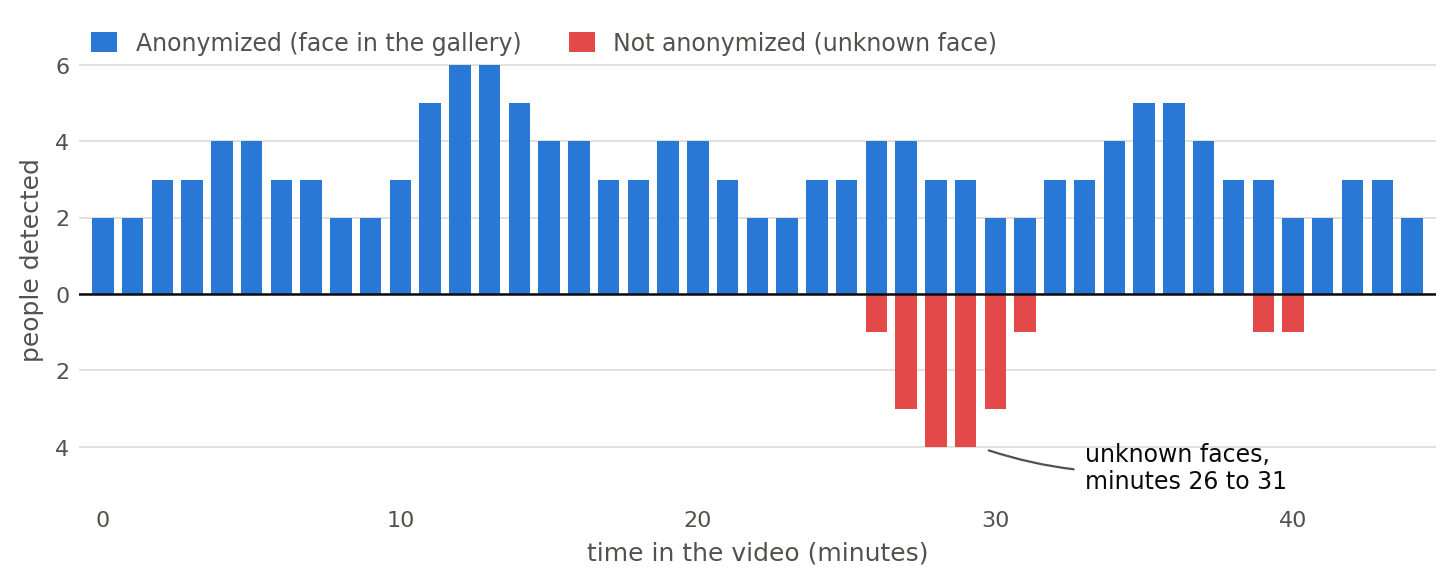
\includegraphics[width=\linewidth]{figures/timeline.png}
\caption{People detected per minute in a 45 minute clip. Above the axis, the faces that
were anonymized. Below it, the faces the system did not recognise.}
\end{figure}

\section*{Q7. (EXTRA) Code snippet: selective anonymization by reidentification}

The snippet below implements Q1: faces come from the detector with a
\textbf{track id}, the embedding is computed \textbf{once per every persons track}, and \textbf{only the people found in the gallery are anonymized} while everybody else
is left without anonymisation. 
\begin{Verbatim}
import cv2
import numpy as np

SIM_THRESHOLD = 0.45   # cosine similarity above which we call it a match
MIN_FACE_PX   = 40     # smaller faces are not reliable enough to identify


def load_gallery(path):
    """Embeddings of the people we have been asked to anonymize."""
    g = np.load(path)                                  # (N, 512)
    return g / np.linalg.norm(g, axis=1, keepdims=True)


def is_target(embedding, gallery):
    """Cosine similarity against the whole gallery in one matrix product."""
    e = embedding / np.linalg.norm(embedding)
    return float(np.max(gallery @ e)) > SIM_THRESHOLD


def anonymize(frame, box):
    x1, y1, x2, y2 = box
    # blur proportional to the face size
    k = max(3, int(0.3 * (x2 - x1)))
    if k % 2 == 0:
        k += 1                                         # GaussianBlur needs an odd kernel
    frame[y1:y2, x1:x2] = cv2.GaussianBlur(frame[y1:y2, x1:x2], (k, k), 0)


def run(stream, detector, embed, gallery_path):
    gallery = load_gallery(gallery_path)
    on_list = {}            # one entry per track: True if that person is in the gallery

    for frame in stream:
        # the detector returns boxes already associated to a track id by the tracker
        for face in detector(frame):
            x1, y1, x2, y2 = face.box
            tid = face.track_id

            # the embedding runs once per track, not once per frame, and only on
            # faces big enough to be identified reliably
            if tid not in on_list and (x2 - x1) >= MIN_FACE_PX:
                on_list[tid] = is_target(embed(frame, face), gallery)

            # only the people in the gallery are anonymized
            if on_list.get(tid, False):
                anonymize(frame, face.box)

        yield frame
\end{Verbatim}

\end{document}
